\section{Evaluation}
\subsection{Experiment platform and implementation}
We implement all algorithms in cuda and cuBlas and evaluate parallel performance on one GPU node which
has two Nvidia M2090 on TACC Lonestar. Sequential implementation is tested on CPU node with
Intel Xeon X5680 3.33GHz processor. We use one GPU to run our experiment. Nvidia M2090 is in Fermi
architecture which supports compute 2.0 capability. The peak single precision floating point performance
is 1331 GFlops. The GPU runs with CUDA 6.5 driver, 5.0
runtime library and Nvidia driver 340.32. For our implementation, we use CUDA 5.0 runtime and cublas API.
During development, we use a local GPU, Nvidia C2075 in Fermi architecture with CUDA 6.5 runtime and cuBl
as API and Nvidia driver 340.29. Peak single precision floating point performance is 1030 GFlops.
We find that our GPU code runs significant faster on our local machine than on TACC. Our GPU code
performance depends on hardware it is running on and version of CUDA API. Later version of compiler may
have optimization that results in this difference. 

\section{Scalability}
We evaluate the scalability of the first parallel algorithm. We cannot control how many CUDA threads it
spawns for algorithms using cuBlas library, so we just compare the performance using the same input size.
With different initial assignment of centroids, algorithms may terminate with different iterations which
impact performance measurement, so we enforce all algorithms run 50 iterations and needs to construct
120 centroids. 

\subsection{Strong scaling}
The input size is 640000 points with 40 dimension. Result is shown in Table~\ref{tab:strong-scaling} and
Figure~\ref{fig:strong_scaling}. 
\begin{table}[ht]
  \centering
  \begin{tabular}{|c|c|c|c|c|c|c|c|}
    \hline
    Number of threads	& 10000	    & 20000	    & 40000	& 80000	& 160000 & 320000	& 640000 \\
    \hline
    Points per thread &	64	      & 32	      & 16	  & 8	    & 4	     & 2	    & 1 \\
    \hline
    Time (s)	   & 14.968109 &	14.739549	& 14.083437	& 13.965568	& 13.923301	& 13.901065	& 13.893361\\
    \hline
  \end{tabular}
  \label{tab:strong-scaling}
  \caption{Strong scaling test for parallel algorithm~\ref{par}}
\end{table}
\begin{figure}[!h]
  \centering
  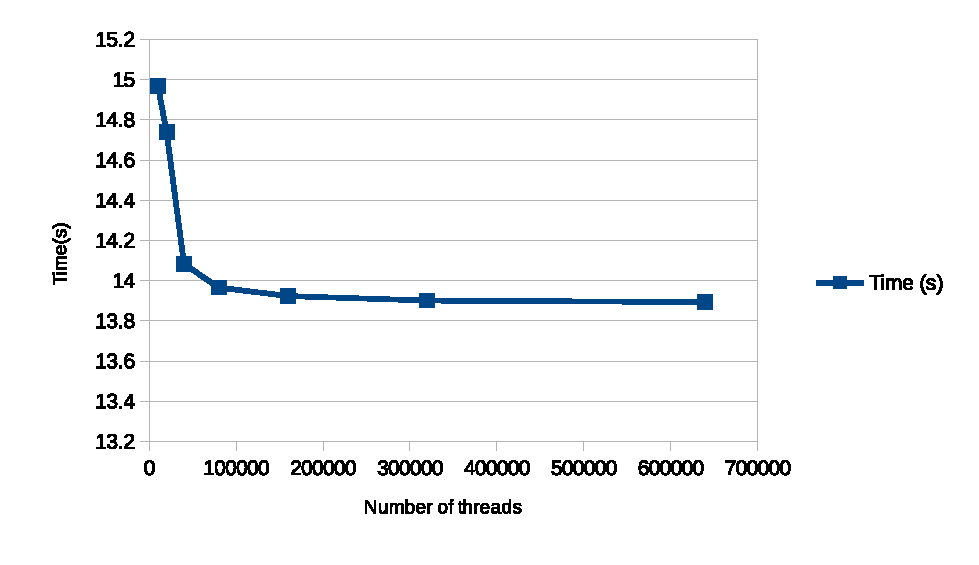
\includegraphics[width=\linewidth]{fig/strong_scaling}
  \caption{Strong scaling test for parallel algorithm~\ref{par}}
  \label{fig:strong_scaling}
\end{figure}

\subsection{Weak scaling}
For weak scaling, we put one point per thread. The number of points equals the total number of threads.
Result is listed in Table~\ref{tab:weak-scaling} and Figure~\ref{fig:weak_scaling}.
\begin{table}[ht]
  \centering
  \begin{tabular}{|c|c|c|c|c|c|c|c|}
    \hline
    Number of points	& 10000	& 20000	& 40000	& 80000	& 160000	& 320000	& 640000 \\
    \hline
    Time (s)	& 5.150253	& 5.334522	& 5.56897	& 6.212595	& 7.27669	& 9.324087	& 13.882712 \\
    \hline
  \end{tabular}
  \label{tab:weak-scaling}
  \caption{Weak scaling test for parallel algorithm~\ref{par}}
\end{table}
\begin{figure}[!h]
  \centering
  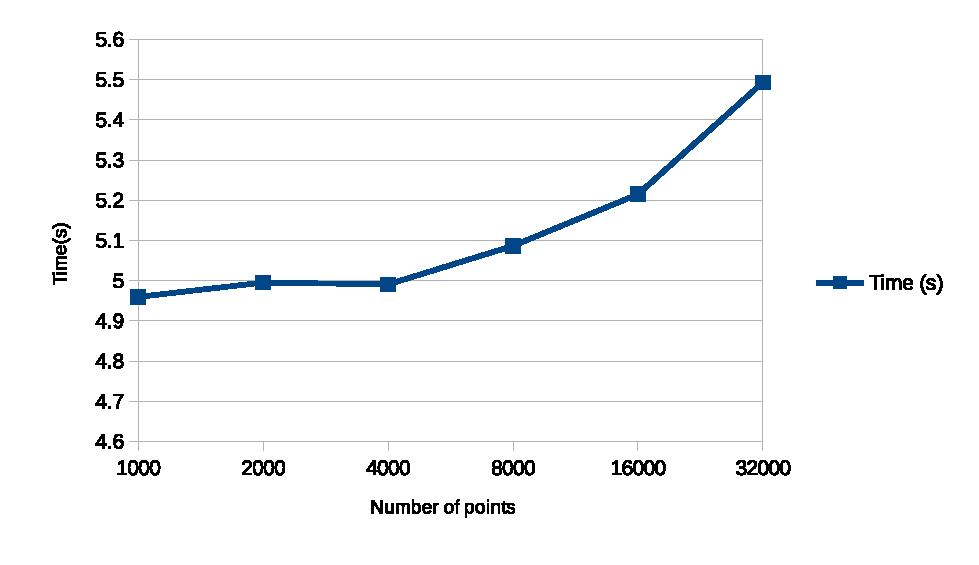
\includegraphics[width=\linewidth]{fig/weak_scaling}
  \caption{Weak scaling test for parallel algorithm~\ref{par}}
  \label{fig:weak_scaling}
\end{figure}

\subsection{Comparison between sequential and parallel algorithms}
We compare sequential algorithm with three versions of parallel algorithm. For each algorithm, it
receives the same input size. For the first algorithm, each thread handles one point. Result is shown in
Table~\ref{tab:comparison} and Figure~\ref{fig:all} and \ref{fig:par}. Parallel v1, v2, v3 correspond to
Algorithm~\ref{par}, \ref{par_m} and \ref{par_vn_m} respectively.   
\begin{table}[!h]
  \centering
  \begin{tabular}{|c|c|c|c|c|c|c|c|c|}
    \hline
    {}& Number of points	& 10000	& 20000	& 40000	& 80000	& 160000	& 320000	& 640000 \\
    \hline
    \multirow{4}{*}{Time(s)}	& sequential	& 13.342	& 26.397	& 52.528	& 105.078	& 210.116	& 420.287	& 840.637 \\
    \cline{2-9}
	  & parallel v1	& 5.150	& 5.335	& 5.569	& 6.213	& 7.277	& 9.324	& 13.883 \\
    \cline{2-9}
	  & parallel v2	& 5.914	& 6.603	& 7.931	& 10.267	& 15.380	& 25.137	& 44.042 \\
    \cline{2-9}
	  & parallel v3	& 5.308	& 5.559	& 6.049	& 6.932	& 8.956	& 12.662	& 20.017 \\
    \hline
  \end{tabular}
  \label{tab:comparison}
  \caption{Comparison of running time between sequential and three versions of parallel algorithms}
\end{table}

\begin{figure}[!h]
  \centering
  \begin{minipage}{.8\textwidth}
    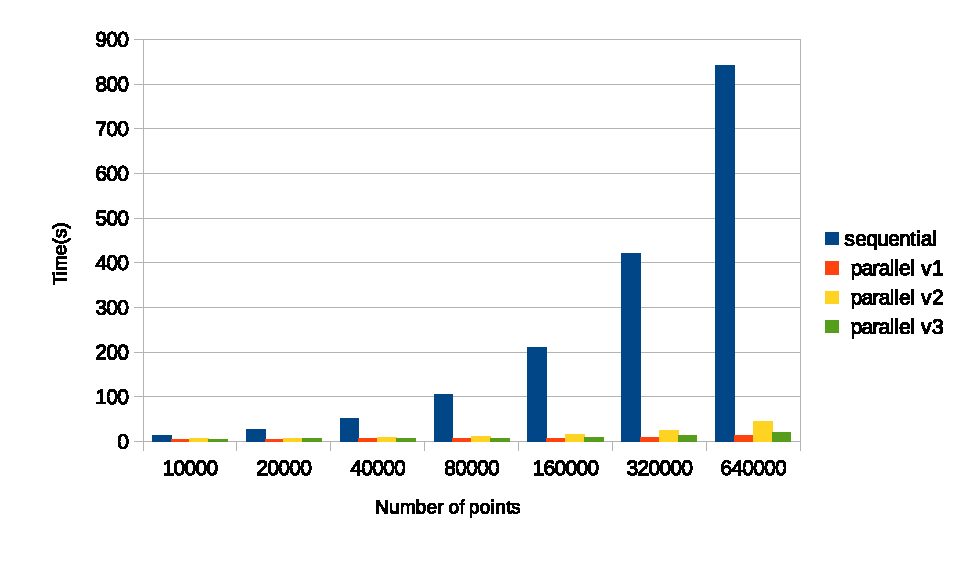
\includegraphics[width=\linewidth]{fig/all_comparison}
    \caption{Comparison of running time between sequential and three versions of parallel algorithms}
    \label{fig:all}
  \end{minipage}
  \begin{minipage}{.8\textwidth}
    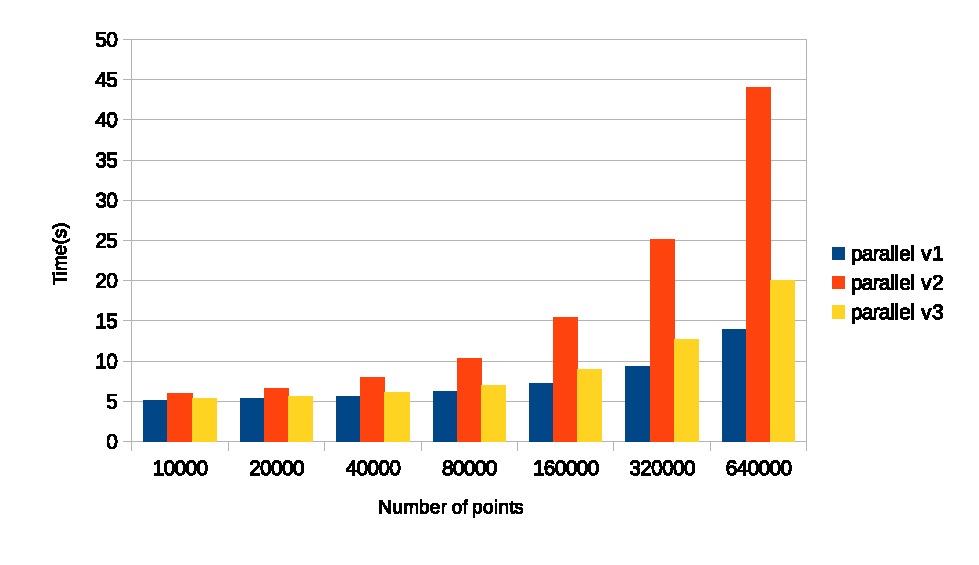
\includegraphics[width=\linewidth]{fig/parallel_algorithm_comparison}
    \caption{Comparison of three parallel algorithms}
    \label{fig:par}
  \end{minipage}
\end{figure}

From Figure~\ref{fig:par}, the hand-turned cuda implementation runs the best, followed by implementation
using cublas matrix-matrix multiplication and using matrix multiplication to calculate vector norm
and the slowest is the one using cublas snorm2 for vector norm. 
